\documentclass[main.tex]{subfiles}

\begin{document}
    \chapter{Introduction}
    \setlength{\epigraphwidth}{0.8\textwidth}
    % \epigraph{
    %         \selectlanguage{greek}
    %         >en p~asi g`ar to~is fusiko~is >'enest'i ti jaumast'on\\
    %         \vspace{0.2cm}
    %         \selectlanguage{english}
    %         In all things of nature there is something of the marvelous
    % }{--- Aristotle, 384-322 BC}
        \epigraph{
            \selectlanguage{english}
            ``You must have chaos within you to give birth to a dancing star''
    }{--- Friedrich Nietzsche, Thus Spoke Zarathustra}
    % \vspace{2cm}


    From the early days when astronomers gazed at the night sky to the present era of cutting-edge instruments and sophisticated computational models, our comprehension of the structure and evolution of stars has grown exponentially. Although many fundamental processes are still poorly understood (e.g., the theory of convection and internal mixing, the effects of rotation and magnetic fields), improvements in both the quantity and quality of observational data, coupled with significant progress in theoretical advancements and the adoption of novel computational techniques, have allowed for an enormous expansion and refinement of both the formal and conceptual basis of the subject.

    In this introductory chapter, we investigate the fundamentals of stellar astrophysics, examining how stars evolve from their formation to their eventual transformation into compact stellar remnants. During this exploration, we focus particularly on neutron stars, which hold significant importance in astrophysics. Formed from the remnants of dying stars, neutron stars serve as unique celestial laboratories, providing valuable insights into the nature of matter and the effects of strong gravity. This dissertation aims to contribute to our understanding of neutron stars by investigating the intricate processes that govern their life cycles, with a specific emphasis on their structure and mass distribution.

    Naturally, it has been necessary to be selective in the material presented. The intention here is to lay the groundwork and provide a succinct overview of key concepts tailored to the dissertation's scope, steering away from an exhaustive exploration of stellar astrophysics principles. However, readers seeking further clarification may find additional resources in classical textbooks that offer extensive coverage across diverse facets of this field \citep[e.g.,][]{Clayton, Prialnik, Eggleton, Kippenhahn, Carroll_Ostlie_2017}.

    
    {\hypersetup{linkcolor=black, pdfborder={0 0 0}}
    \adjustmtc
    \adjustmtc
    \minitoc
    \newpage
    }
    
    
    
    \section{A Brief Introduction to Stellar Structure \& Evolution}\label{sec:ch1:intro}
    From humanity's standpoint, stars often appear as timeless entities, seemingly having existed for eternity and destined to persist indefinitely in the vast expanse of the Universe. This perception, however, is an illusion, stemming from the limited time span during which we observe these celestial bodies in relation to their overall lifetime. In reality, stars undergo the complex processes of birth, evolution, and eventual demise within the cosmic landscape, unfolding over timescales beyond human intuition. To comprehend the evolution of stars over time, observational studies inherently rely on short-term measurements taken from extensive populations.
    Consider the analogy of a paleoanthropologist studying the biological and cultural evolution of humans throughout history. With the first appearance of Homo sapiens believed to have occurred approximately \SI{200000}{years} ago, the only viable method for such a study is through the examination of a large population of fossil records and archaeological evidence spanning different evolutionary stages.

    Given a large sample of stars, we may construct the so-called \textit{``Hertzsprung-Russell diagram''} (H-R diagram), where stars' luminosity is plotted against their effective surface temperature\footnote{It is worth noting that variations of the H-R diagram exist. In alternative forms, the diagram may employ color, magnitude, or spectral type on its axes. For instance, a Color-Magnitude Diagram (CMD) is a variation that plots stars based on their color and magnitude, providing insights into stellar populations and evolutionary stages based on these observable characteristics.}, an example of which can be seen in Fig.~\ref{fig:hrd_gaia}. This diagram provides a visual representation of stellar characteristics, allowing us to organize and analyze large populations of stars simultaneously. Through the H-R diagram, stars can be classified based on their luminosity, temperature, and evolutionary stage, providing a comprehensive snapshot of various stellar life cycles. Much like the paleoanthropologist's careful examination of diverse fossil records, the H-R diagram offers astronomers a panoramic view of stellar evolution, enabling them to unravel the mysteries embedded in stellar dynamics.

    \begin{figure}[h!]
        \centering
        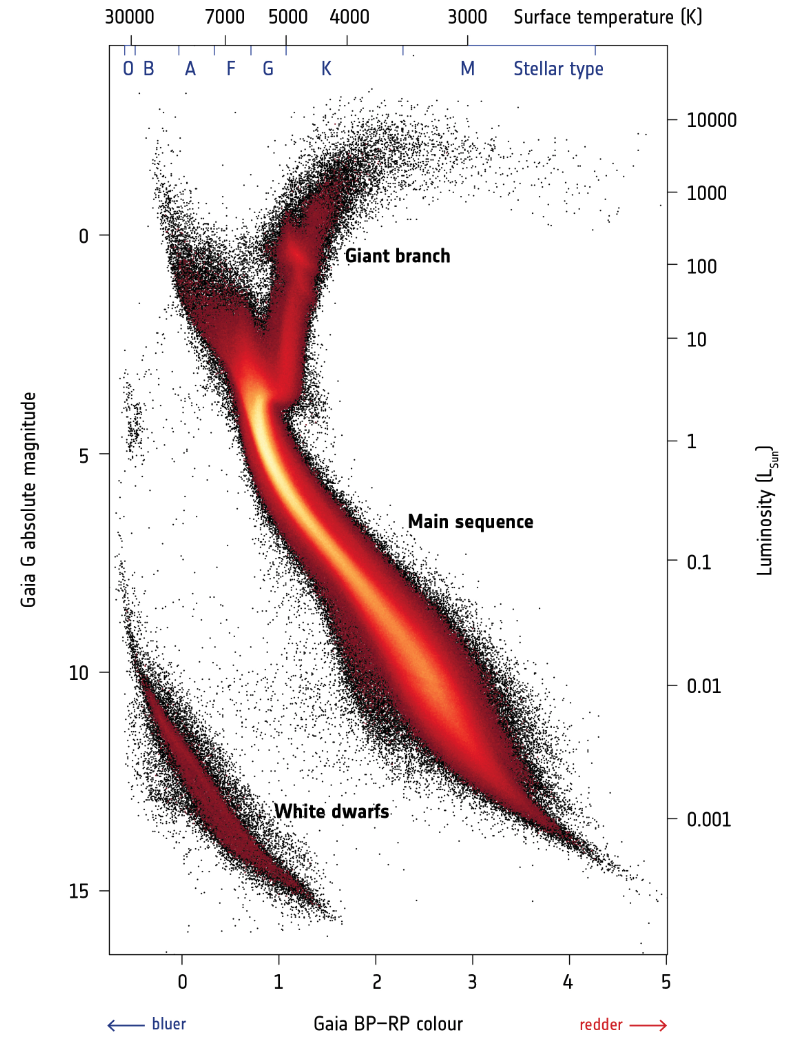
\includegraphics[scale=0.25]{figures/chapter1/hrd_gaia.png}
        \caption{Hertzsprung-Russell diagram obtained by a selection of stars from the second release catalogue of ESA's Gaia satellite. Copyright: \href{https://sci.esa.int/web/gaia/-/60198-gaia-hertzsprung-russell-diagram}{ESA/Gaia/DPAC}.}
        \label{fig:hrd_gaia}
    \end{figure}

    Upon a casual observation of Fig.~\ref{fig:hrd_gaia}, it becomes evident that stars are not randomly distributed on the H-R diagram but instead cluster, forming distinct structures primarily based on their masses, chemical composition, and evolutionary stage. The most prominent of these structures is a large collection of stars forming a diagonal stripe known as the \textit{``main sequence''}. Above the main sequence lies another feature referred to as the \textit{``giant branch''}, while below the main sequence, stars are distributed on the left-hand side, forming a group of objects known as \textit{``white dwarfs''}. The presence of these structures on the H-R diagram implies the existence of underlying physical laws governing these observational characteristics, which will hopefully become apparent in the following sections.

    

    \newpage
    \subsection{Stars in Isolation: From Birth to Death}
    This section provides a broad overview of the life cycle of individual stars, encompassing their birth through their eventual demise. While we will touch upon the processes occurring within the stellar interior, such as energy generation mechanisms, the significant impact of other factors, such as mixing and rotation, on stellar evolution will be explored in more detail in a subsequent section.
    
    \subsubsection{Star formation}
    The life of a star is the story of a cosmic tug-of-war between gravity and the star's internal pressure. This story begins within giant molecular clouds, an agglomeration of interstellar gas and dust. These molecular clouds are often composed of hydrogen molecules, helium, and trace amounts of other elements\footnote{In astronomy, elements heavier than helium are commonly grouped under the term ``metals'', although this classification doesn't necessarily reflect their chemical properties. The abundance of these heavier elements within celestial structures, such as stars, is quantified by the term ``metallicity''.}, serving as the cosmic nurseries where stars are born (see Fig.~\ref{fig:rho_ophiouchi}).
    Initially, the molecular cloud is in a state of equilibrium, where thermal motions, driven by temperature, work to resist the force of gravity that seeks to collapse the cloud. The interplay between these opposing forces is described by the \textit{virial theorem} which, under the assumption that the cloud behaves as an ideal gas, takes the form:
    \begin{equation}\label{eq:virial}
        2E_\mathrm{kin} + E_\mathrm{gr} = 0,
    \end{equation}
    where $E_\mathrm{kin}$ is the kinetic energy and $E_\mathrm{gr}$ is the gravitational potential of the system. For as long as this equation holds true, the system will neither expand nor collapse. If the kinetic energy term dominates, then the thermal pressure overcomes the gravitational attraction and the system will expand. On the other hand, if the gravitational potential term dominates, the system will contract on the free-fall (dynamic) timescale:
    \begin{equation}\label{eq:dynamical_timescale}
        \tau_\mathrm{ff} \propto (G\bar{\rho})^{-1/2},
    \end{equation}
    i.e., the characteristic time that would take a body to collapse under its own gravity. Here $G$ is the gravitational constant and $\bar{\rho}$ is the average density of the cloud. Owing to the extremely low densities that characterize molecular clouds, the free-fall timescale is of the order of million of years.

    \begin{figure}[t]
        \centering
        \includegraphics[scale=0.07]{figures/chapter1/Rho_Ophiuchi_cloud_complex.jpg}
        \caption{The $\rho$-Ophiouchi cloud complex, one of the closest star-forming regions to our Solar System, located at the constellation of Ophiuchus. The photograph is a compilation of distinct exposures gathered by the James Webb Space Telescope through the utilization of the NIRCam instrument. Copyright: \href{https://www.esa.int/ESA_Multimedia/Images/2023/07/Rho_Ophiuchi_cloud_complex}{NASA, ESA, CSA}.}
        \label{fig:rho_ophiouchi}
    \end{figure}

    By applying the virial theorem, it can be shown that there exists a critical mass threshold, known as the ``Jeans mass'' ($M_J$), which characterizes the point at which self-gravity becomes dominant, overcoming thermal pressure. The Jeans mass is expressed by the formula:
    \begin{equation}\label{eq:jeans_mass}
        M_J \approx \left(\frac{3}{4\pi \rho}\right)^{1/2} \left(\frac{5kT}{G\mu m_H }\right)^{3/2}, 
    \end{equation}
    where $k$ is the Boltzmann constant, $T$ is the temperature of the molecular cloud, $G$ is the gravitational constant, $\rho$ is the density of the cloud, $\mu$ is the mean molecular weight, and $m_H$ denotes the mass of the hydrogen atom.

    Star formation begins as portions of the molecular cloud undergo gravitational collapse, triggered by small irregularities in the distribution of matter. Such density inhomogeneities may be induced by turbulence or external factors, like shockwaves from nearby supernovae and spiral density waves, ultimately leading to gravitational instabilities. Consequently, the molecular cloud fragments into denser regions, surpassing the Jeans mass. These more condensed areas, known as cloud cores, become the sites where individual stars are born and take shape.

    As a molecular cloud core contracts under the influence of gravity, it undergoes an initial phase of isothermal collapse. This phase results in the formation of a \textit{protostellar disk} and, subsequently, a \textit{protostar} at its center. Material continues to accrete onto the protostar, while the surrounding protostellar envelope gradually dissipates over time. This phase plays a critical role in determining the initial mass and angular momentum of the nascent star.
    Throughout this collapse, the core's temperature remains relatively constant due to efficient cooling mechanisms. However, as the density increases, the opacity of the material undergoes a change. In the early stages, when the core is less dense, it is optically thin, allowing radiation to easily escape. However, as the density rises, the core becomes optically thick, hindering radiation from propagating through the increasingly dense material. This shift in opacity significantly influences the thermal balance within the collapsing core\footnote{During this process, energy is generated via the Kelvin-Helmholtz mechanism. The gravitational potential energy liberated due to contraction is radiated away in the form of light.}.
    
    As the core progresses through its evolution, opacity continues to impact its thermal properties. At higher densities, the core transitions from an isothermal collapse to an adiabatic collapse (where cooling can be ignored), leading to a more substantial rise in temperature due to increased opacity. This gives rise to the birth of a protostar within the dense core. The protostar subsequently undergoes further evolution along the Hayashi track\footnote{A trajectory on the Hertzsprung-Russell diagram showcasing the thermal evolution of the protostar during contraction until hydrostatic equilibrium is achieved via central nuclear fusion.}, contracting and heating until the conditions are suitable for the ignition of hydrogen in its center ($T_c \sim 10^7\,\text{}K$). The onset of sustained nuclear fusion in the protostar's core results in the establishment of hydrostatic equilibrium and prevents further collapse. A new star has just been born and has joined the main sequence as a ``\textit{zero age main sequence}'' (ZAMS) star!
    

    \subsubsection{Evolution during the main sequence}
    During the main sequence phase, all stars exhibit a fundamental set of characteristics that define this stable stage in their evolution. Central to this phase is the process of hydrogen burning in the star's core, which involves fusing hydrogen nuclei together to form helium. This nuclear fusion generates a continuous release of energy, establishing a delicate equilibrium between the gravitational forces 
    and the outward pressure gradient generated by the ongoing fusion reactions.

    Two primary mechanisms govern central hydrogen burning in stars: the proton-proton (pp)-chain and the carbon-nitrogen-oxygen (CNO) cycle. In the pp-chain, predominant in lower-mass stars like the Sun, hydrogen nuclei (protons) undergo a series of fusion reactions, ultimately resulting in the conversion of four protons into one helium nucleus, liberating energy in the process. Although the net reaction can be written as:
    \begin{equation}
        \label{eq:pp-chain}
        \mathrm{4\,^1H \longrightarrow \,^4He + 2\,e^+ + 2\,\nu_e + Q(\sim 26.7\,MeV)},
    \end{equation}
    it should be noted that this chain of reactions involves various intermediary steps, including the formation of deuterium and helium-3 as can be seen in Fig.~\ref{fig:pp_cno}.

    \begin{figure}[th!]
        \centering
        \begin{subfigure}{.5\textwidth}
        \centering
        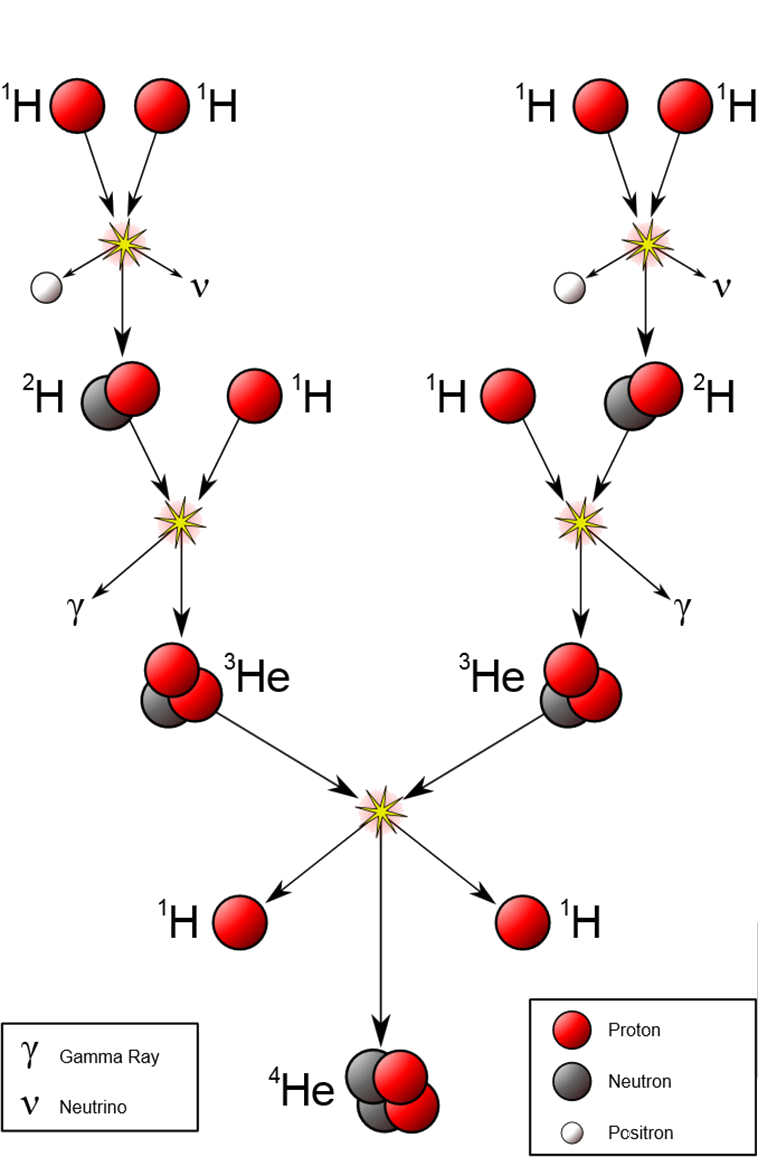
\includegraphics[scale=0.25]{figures/chapter1/pp-chain.png}
    \end{subfigure}%
    \begin{subfigure}{.5\textwidth}
        \centering
        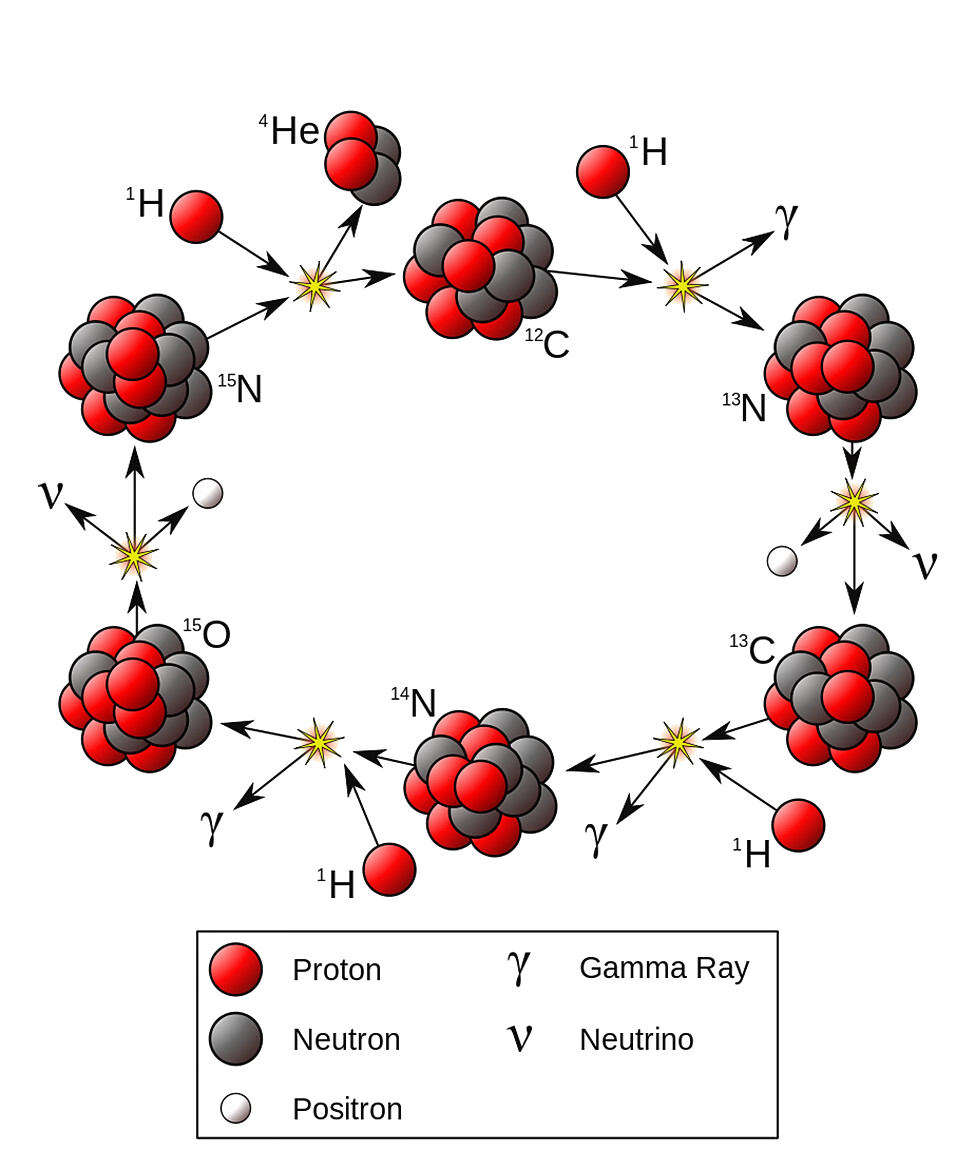
\includegraphics[scale=0.2]{figures/chapter1/cno-cycle.png}
    \end{subfigure}
        \caption{Schematic illustration depicting the primary mechanisms driving energy generation in main sequence stars. On the left, the proton-proton chain is portrayed, while on the right, the CNO cycle is presented. Credit: \href{https://supernova.eso.org/}{ESO Supernova}.}
        \label{fig:pp_cno}
    \end{figure}
    
    Conversely, in higher-mass stars, the CNO cycle becomes a dominant contributor to central hydrogen burning. This cycle involves catalytic fusion reactions facilitated by carbon, nitrogen, and oxygen isotopes acting as catalysts\footnote{The net result of the CNO cycle is the same, regardless of which of these elements initiates the process.}. The CNO cycle is more temperature-sensitive than the pp-chain and becomes increasingly significant in hotter and denser stellar cores. It offers an alternative pathway for hydrogen fusion, enhancing the efficiency of energy production in more massive stars.

    Nevertheless, regardless of the energy generation mechanism, whether it be the pp-chain or the CNO cycle, the temperature and density within the star remain nearly constant until the depletion of hydrogen. The duration of hydrogen burning is determined by the star's mass and luminosity:
    \begin{equation}
        \label{eq:nuclear_timescale}
        \tau_\mathrm{nuc} = \phi f \frac{Mc^2}{L},
    \end{equation}
    known as the ``\textit{nuclear timescale}'', where $M$ is the total mass of the star, $L$ is it's surface luminosity, $c$ is the speed of light, $f$ is the fraction of the total mass of the star that participates in nuclear burning, and $\phi$ is the fractional mass difference of the reaction, i.e., the fraction of the mass that is being converted into energy in each reaction (for hydrogen burning, $\phi \simeq 0.7\%$). Massive stars are vastly more luminous than lower-mass stars; hence, the nuclear timescale on which they burn their hydrogen supplies is of the order of a few million years. On the other hand, the lowest-mass stars may remain in the main sequence for a period that may exceed the current age of the universe. In both cases, however, stars spend most of their lives in this stable phase, which explains the prominence of the main sequence feature on the H-R diagram.
    


    \subsubsection{Evolution after the main sequence}
    After the eventual exhaustion of their energy source, stars that exit the main sequence feature an inert core composed mainly of helium engulfed in a hydrogen-rich mantle. Without the nuclear reactions to provide an outward pressure to counterbalance gravity, the stars' core falls out of equilibrium and begins to contract. As the temperature increases, the conditions become favorable for the ignition of hydrogen in the outer layers surrounding the inert helium core. This external shell burning generates enough energy to cause the layers above it to expand; the radius of the star grows dramatically and it's surface effective temperature decreases, i.e., it appears redder. The star has transformed into a red giant and starts ascending the red giant branch on the H-R diagram.

    In spite that shell hydrogen burning has restored hydrostatic equilibrium by providing support to the outer layers of the star, the inert helium core continues to contract and heat up.
    This transitional stage represents a crucial point in stellar evolution, giving rise to distinct pathways for stars with different masses. In lower-mass stars, the core contracts until electron degeneracy pressure becomes the primary force preventing further collapse instead of thermal pressure. This pressure arises from the Pauli exclusion principle, which prohibits two fermions, such as electrons, from simultaneously occupying the same quantum state. The hydrogen-burning layer above the inert core produces more helium via one of the processes we described earlier. In turn, this helium is accumulated on top of the helium core, allowing it to grow in mass. If the core reaches a critical mass of approximately $0.4\msun$, then the conditions for initiating core helium burning are fulfilled. Because the core is composed of degenerate matter, when the core temperature reaches a critical level, around 100 million Kelvin, a sudden and explosive ignition of helium occurs in a process known as the ``\textit{helium flash}''. This ignition is not gradual like in earlier burning stages; instead, it is rapid and releases an enormous amount of energy. 
    
    The helium flash marks the onset of helium burning, converting helium into carbon and oxygen via the triple-alpha process\footnote{This is the mechanism in which three helium nuclei (alpha particles) undergo a two-step fusion process, ultimately yielding carbon. Subsequent fusion involves carbon combining with another helium nucleus to generate oxygen.}.
    Although the helium flash is a dramatic event, it does not lead to a visible explosion on the stellar surface. The outer layers of the star absorb the released energy, causing the star to expand and readjust its structure. After the helium flash, the star settles into a more stable phase of helium shell burning, continuing its evolution towards the horizontal branch\footnote{Notice that stars on the horizontal branch may have two energy sources: core helium burning and shell hydrogen burning.} on the H-R diagram. The duration of shell hydrogen burning and core helium burning is very short compared to the duration of the main sequence. This is the reason why there are relatively fewer red giants than main sequence stars.

    In the case of massive stars, the evolution leading up to this stage follows a similar trajectory. The key distinction lies in the fact that their inert helium core meets the criteria for core helium burning before gravitational contraction induces degeneracy. Consequently, the initiation of helium burning in their cores is a more gradual process, without giving rise to a helium flash. From this point onwards, the evolution of low- and intermediate-mass stars and massive stars becomes significantly different. 
    
    In the aftermath of core helium depletion, if stars possess sufficient mass, they undergo successive burning phases, transitioning from carbon to neon, then oxygen, and finally silicon. However, this burning sequence ceases upon the formation of an iron core at the star's center. Iron-group elements exhibit the highest binding energy per nucleon, rendering any nuclear reaction involving them endothermic. Consequently, these reactions cannot contribute to the pressure gradient crucial for counteracting gravitational collapse, and all stars that develop such dense iron cores are doomed. The structure of such massive stars during these final stages resembles that of an onion or the concentric rings found in tree barks. Much like the rings in a tree, each stellar layer represents a distinct phase of nuclear burning in the star's evolutionary journey (see Fig.~\ref{fig:stellar_structure}).
    \begin{figure}[hb!]
        \centering
        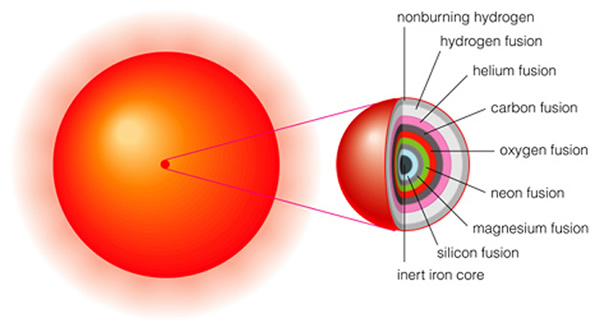
\includegraphics[scale=0.5]{figures/chapter1/high-mass-star-struct.jpeg}
        \caption{Illustration of the inner structure of a massive star before core-collapse. Credit: \href{http://astronomy.nmsu.edu/tharriso/ast110/}{Thomas Harrison | New Mexico State University}.}
        \label{fig:stellar_structure}
    \end{figure}
    Sooner than later, the iron core will collapse and trigger a supernova explosion, known as a ``\textit{core-collapse supernova}'', leaving behind a remnant in the form of a \textit{neutron star} or a \textit{black hole}.
    
    Lower-mass stars, on the other hand, have a different fate; since their cores never reach a high enough temperature to initiate carbon burning, they contract, developing a degenerate, inert core composed primarily of carbon and oxygen. The outer envelope, opposing the contraction of the inert core, expands, causing the star to cool as it enters the \textit{asymptotic giant branch} (AGB) in the H-R diagram.
    Simultaneously, strong stellar winds cause the outer layers to expel, forming a \textit{planetary nebula} and exposing the degenerate core. This naked core, known as a \textit{white dwarf}, is the final remnant left behind by such stars and no longer undergoes nuclear reactions but simply gradually cools down by radiating the residual heat.


    \subsubsection{Mixing in stellar interiors}
    The interior of a star is far from quiet. Equipped with a better understanding of how stars evolve, it is time to dive a little deeper into the more intricate dynamical processes that play a crucial role in their evolution. Here we will briefly present four fundamental mixing mechanisms caused by various instabilities.

    One of the most important mixing mechanisms that takes place in the stellar interior is that of \textit{convection}. It occurs when temperature variations across different layers induce density fluctuations, leading to buoyancy-driven fluid flows. This buoyancy-driven motion efficiently transports heavy elements through bulk motions, a phenomenon known as ``\textit{dredge-up}'', leading to the redistribution of material and energy. Essentially, a heated fluid parcel ascends due to buoyancy forces, while a colder parcel descends, taking its place. This convective process profoundly influences the star's structure, impacting phenomena like nucleosynthesis and magnetic field generation. Figure~\ref{fig:sun_granulation} depicts the granulation on our Sun's photosphere---a prominent illustration of the consequences of convection.
    
    \begin{figure}[ht!]
        \centering
        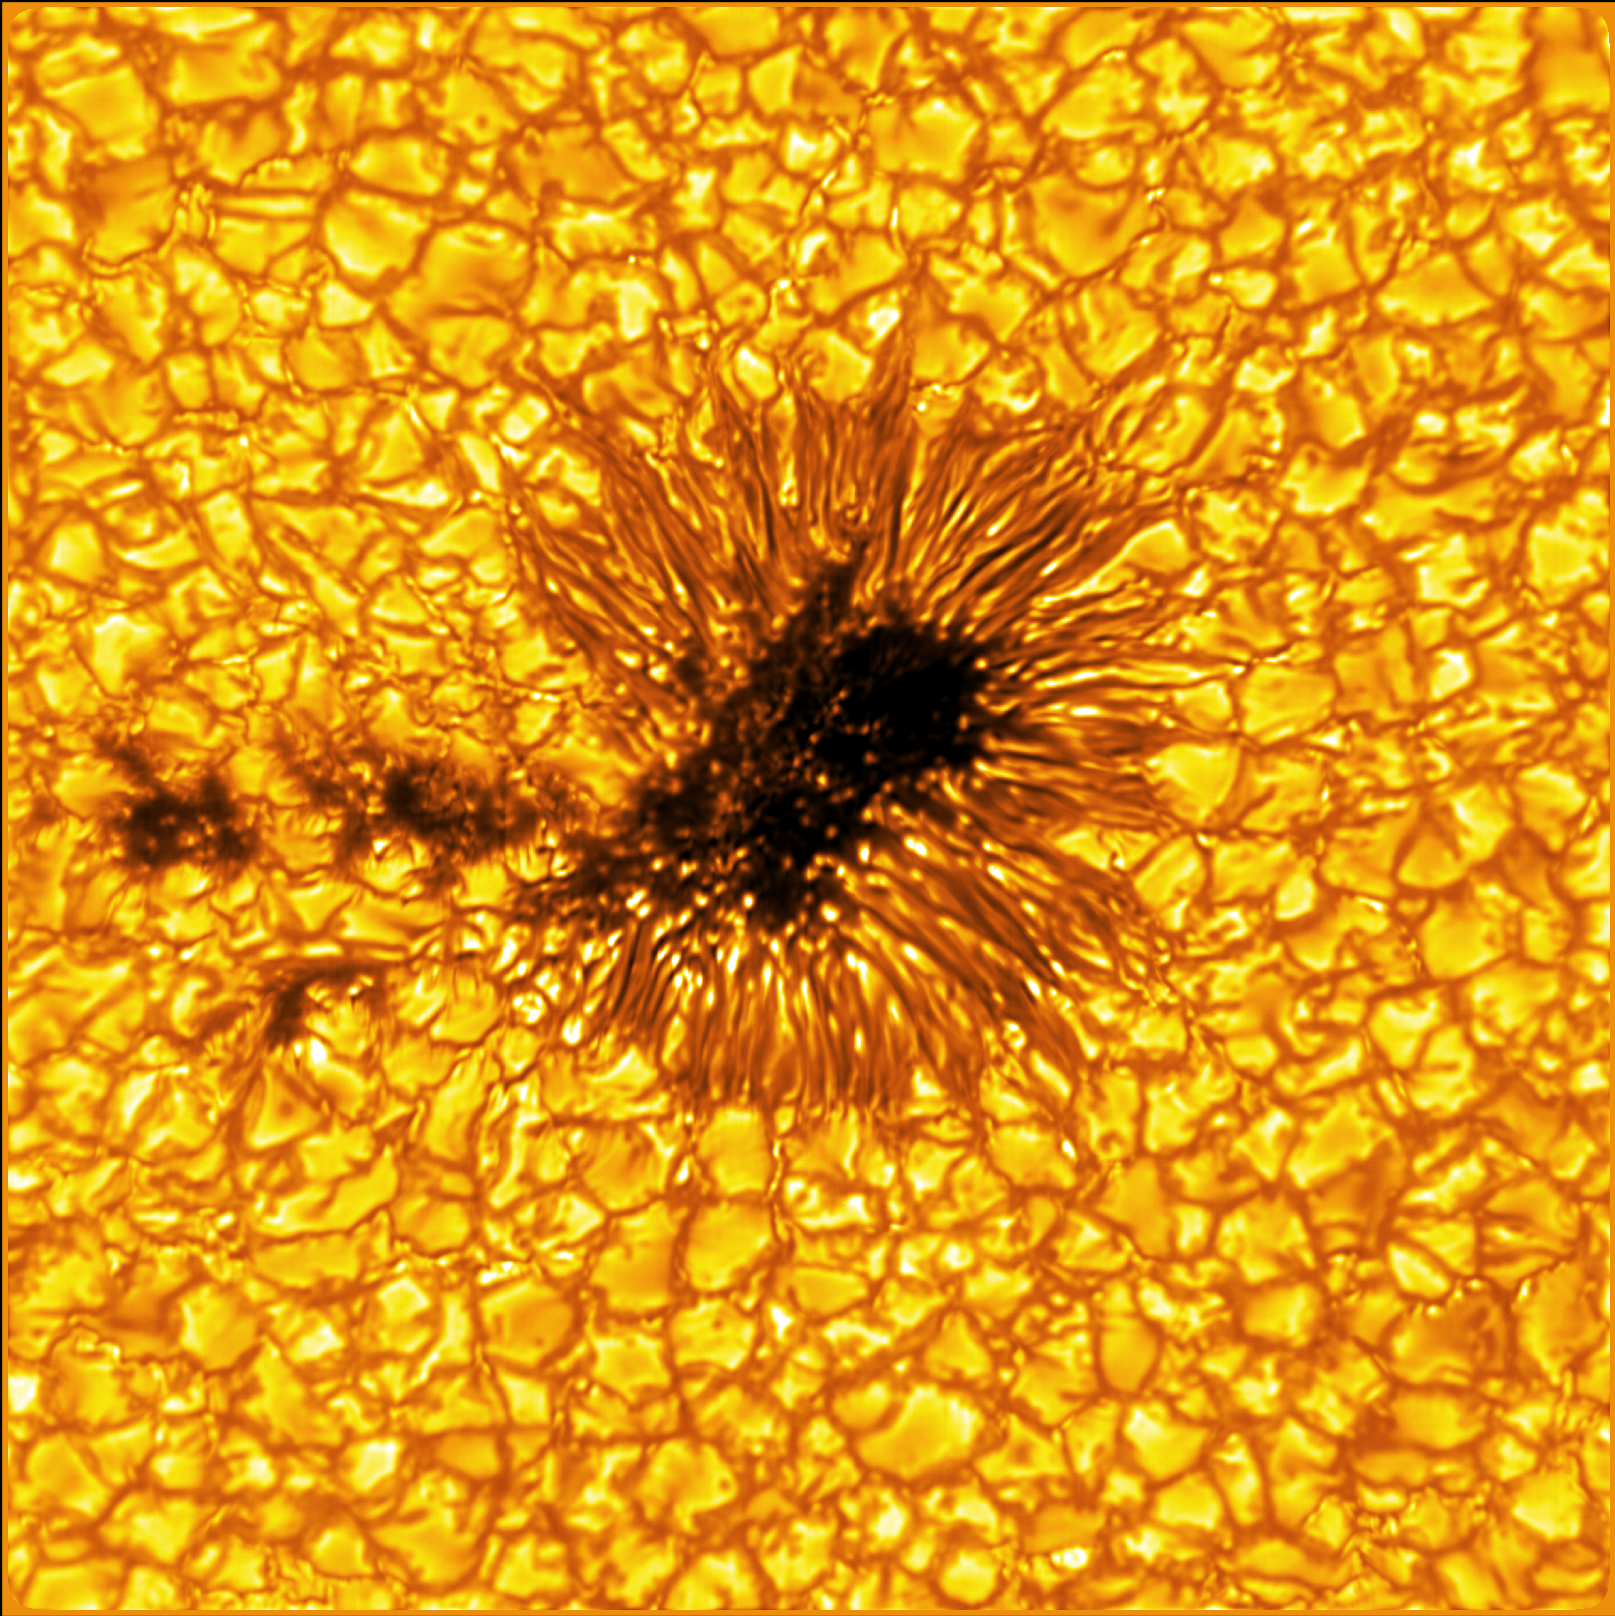
\includegraphics[scale=0.4]{figures/chapter1/sun_granulation.png}
        \caption{A captivating view of the Sun's photosphere revealing distinct granulations scattered across its surface. In the center, a large black sunspot stands out, its darkness attributed to a lower temperature caused by intense magnetic fields that disrupt the convective transfer of heat. This stark contrast highlights the dynamic interplay of convective processes and magnetic fields on the solar surface. Copyright: \href{https://nso.edu/}{National Solar Observatory}.}
        \label{fig:sun_granulation}
    \end{figure}

    The stability of a layer against convection is determined by the \textit{Ledoux} criterion:
    \begin{equation}\label{eq:ledoux}
        \nabla_{\text{rad}} < \nabla_{\text{ad}} - \frac{\phi}{\delta} \nabla_{\mu}
    \end{equation}
    In the case of chemically homogeneous layers ($\nabla_{\mu} = 0$), reduces to the \emph{Schwartzschild} criterion:	
    \begin{equation}\label{eq:schwarzschild}
        \nabla_{\text{rad}} < \nabla_{\text{ad}}
    \end{equation}
    Here, $\nabla_\mathrm{rad}$ represents the radiative temperature gradient describing the logarithmic temperature variation with depth when energy is transported by radiation, $\nabla_\mathrm{ad}$ is the adiabatic temperature gradient defined similarly to $\nabla_\mathrm{rad}$ but for adiabatic compression or expansion, and $\nabla_\mu$ is the composition gradient accounting for variations in chemical composition within the medium.
    
    Modeling convection in astrophysical contexts is a notoriously difficult problem and poses significant challenges due to the complex, turbulent nature of convective flows. The inherent non-linearity and multi-scale behavior of convective processes make their accurate representation in numerical simulations demanding. One widely employed approach is the \textit{Mixing Length Theory} (MLT), which simplifies convective dynamics by introducing a characteristic length scale to describe the convective cells' average size and behavior. While MLT has been successful in certain applications, it has limitations in capturing the full complexity of convection, especially in regions with varying conditions. As a result, convection is often treated as a diffusive process in computational models, wherein the convective transport of energy, momentum, and chemical species is approximated using diffusion equations. This simplification facilitates numerical simulations but may overlook finer details of convective behavior, introducing a lot of uncertainties in our stellar evolution models.

    Another mixing process observed in stellar interiors is called \textit{semi-convection}, which is characterized by an intermediate state between full convection and radiative diffusion. This phenomenon occurs in regions where convective instability interacts with stratified layers, i.e. in regions that are stable to Ledoux criterion but unstable to Schwarzschild \citep[see][]{spruit:semiconvection}. Semi-convection contributes to the transport of both chemical elements and angular momentum, influencing the internal rotation profiles of stars and impacting their overall evolution.

    As we mentioned, the boundaries of a convective zone are determined by the Ledoux or Schwarzschild criteria. Nevertheless, \textit{convective overshooting} extends the impact of convective zones beyond their formal boundaries. As convective cells reach the boundaries of a convective region, they may overshoot and penetrate into adjacent stable layers due to their inertia until they lose all of their momentum. This overshooting process has implications for the extent of mixing in the stellar interior, affecting the transport of elements and altering the size of convective cores in evolving stars.
    
    Last but not least, in certain stellar environments, a phenomenon known as \textit{thermohaline} mixing manifests when there is a decrease in molecular weight with depth. This scenario often arises in binary systems undergoing accretion, creating stratified layers such as a helium layer overlying a hydrogen-rich one. As a consequence, the heavier elements tend to sink while the lighter materials ascend, leading to a restructuring of the mean molecular weight.

    

    \subsubsection{Stellar rotation}
    Thus far, we have silently operated under the assumption that the overview of stellar evolution provided relates solely to spherically symmetrical, non-rotating stars. However, rotation constitutes a crucial factor that profoundly impacts the evolution of stars and deserves to be discussed separately. 

    The inclusion of rotation introduces an---even more---dynamic aspect to stellar evolution, influencing various processes such as angular momentum transport, magnetic field generation, and the overall structure of a star. As stars form from rotating molecular clouds, the conservation of angular momentum plays a pivotal role in shaping their subsequent evolution. The rotation rate affects the size, shape, and internal distribution of matter within a star, influencing its overall stability and lifespan.

    Rotation induces various instabilities that significantly influence the mixing processes and internal dynamics of stars. The Eddington-Sweet circulation, for instance, arises due to the interaction between rotation and density gradients, leading to meridional flows that impact the transport of heat and various isotopes within the stellar interior. The dynamical shear instability and secular shear instability are additional rotational instabilities that can affect the internal shear profile of a star, influencing its overall stability and evolution. Additionally, the interplay between rotation and magnetic fields gives rise to phenomena like the solar dynamo, influencing the generation and modulation of the star's magnetic activity.

    Understanding the role of rotation-induced instabilities in stellar evolution is crucial for deciphering the observed diversity in stellar properties and behaviors. As stars age, their rotation rates can change due to processes like stellar winds and mass loss, further impacting their evolution. Therefore, a comprehensive exploration of stellar evolution necessitates a detailed examination of the influence of rotation and the associated instabilities.

    \subsubsection{Stellar winds}
    The interior of a star is not the only site of great turmoil that determines its evolution. The surface of a star is also a violent environment that can influence its surroundings beyond its own luminous boundaries. One fundamental phenomenon within this narrative is that of \textit{stellar winds}---the continuous flow of gas and charged particles ejected from the upper atmospheres of stars. For single stars, stellar winds are a primary factor in mass loss, especially in the later stages of their lives, affecting their mass, luminosity, and size over time. To make things even more interesting, these winds also contribute to the chemical enrichment of the interstellar medium, as material from the star is dispersed into space.

    The intensity and composition of stellar winds depend on factors such as the star's mass, temperature, and evolutionary stage. For massive stars, such as O-type and B-type stars, mass loss is primarily driven by radiation pressure, where photons exert a force on the star's outer layers, propelling them outward. These winds can be extremely powerful, capable of removing significant portions of the star's mass over its lifetime.
    This process is less significant in lower-mass stars, such as the Sun, where stellar winds are driven by other mechanisms, such as magnetic fields and acoustic waves interacting with the stellar atmosphere. In this case, stellar winds are less intense but still contribute to the star's mass loss and the shedding of angular momentum, impacting the star's rotation rate, particularly during the red giant phase. Overall, the effect of stellar winds is evident in the H-R diagram, where stars that have lost significant mass through stellar winds occupy different positions than they would have otherwise.

    Empirical relations have been established to quantify mass loss rates from the observational spectra of stars. Observations at various wavelengths, from X-ray to radio, allow us to study the properties of stellar winds, including their speed, density, and composition. One of the key empirical relations is the correlation between the star's luminosity and its mass loss rate, often expressed in the form of power laws. These relations are derived from observations of spectral lines that are sensitive to the velocity and density of the wind. For example, the P Cygni profiles observed in ultraviolet spectra are indicative of strong stellar winds in massive stars \citep[e.g.][]{israelian:ssr99}. These empirical relations are critical for modeling the evolutionary tracks of stars, as they provide a means to incorporate mass loss due to stellar winds into stellar evolution codes.

    

    \subsection{Stellar Remnants in a Nutshell}\label{sec:ch1:remnants}
    Following the cessation of nuclear fusion, stars transition into one of three end states: white dwarfs, neutron stars, or black holes, depending on their initial mass and subsequent evolutionary pathways. In what follows, we briefly discuss the characteristics and formation mechanisms of these stellar remnants.
    
    \subsubsection{White Dwarfs}
    White dwarfs are formed from the remnants of stars that have exhausted their nuclear fuel. As presented in the previous section, a star burns through its hydrogen in a process known as nuclear fusion, creating helium and later heavier elements up to iron in more massive stars. Once the nuclear fuel is depleted, and if the star's mass is below approximately $8\msun$, it will not undergo a supernova explosion. Instead, it sheds its outer layers, creating a planetary nebula, while the core contracts under gravity. This core remnant is what we call a white dwarf. It is characterized by its incredibly dense composition, primarily consisting of carbon and oxygen, which results from the fusion of helium in its final burning phase.  In some cases, particularly in more massive white dwarfs that have a mass closer to the Chandrasekhar limit (see below), heavier elements like neon and magnesium can be found.

    In the absence of significant thermonuclear reactions, their energy emission is solely due to the residual thermal energy left over from the star's previous nuclear burning phase, which gradually radiates away, causing the white dwarf to cool and dim over time\footnote{The low-temperature, low-luminosity of aged white dwarfs is the reason they occupy the lower left corner in the H-R diagram.}. However, without thermonuclear reactions to provide the necessary pressure gradient to support white dwarfs against gravity and establish hydrostatic equilibrium, one may wonder how these objects exist. The short answer is that the structural integrity of a white dwarf is achieved through electron degeneracy pressure rather than the thermal pressure found in most stars. 

    \begin{figure}[th!]
        \centering
        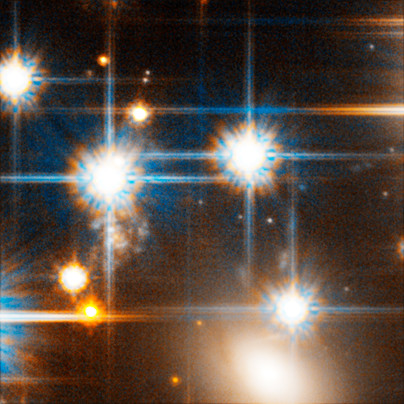
\includegraphics[scale=0.6]{figures/chapter1/wd_ngc6397.jpeg}
        \caption{The photograph captures a faint, cooling white dwarf (center of the image between the two brighter stars) as seen by the Hubble Space Telescope in the globular cluster NGC 6397. Credit: \href{https://esahubble.org/images/heic0608c/}{NASA, ESA and H. Richer (University of British Columbia)}.}
        \label{fig:wd_ngc6397}
    \end{figure}
    
    In the dense core of a white dwarf, electrons are packed so closely together that they are forced into a state of degeneracy, a quantum mechanical effect that arises from the Pauli exclusion principle. This degeneracy pressure is described by a polytropic equation of state, which can be approximated by:
    \begin{equation}\label{eq:polytropic_eos}
        P \simeq K \rho^\gamma,
    \end{equation}
    where $\rho$ is the density of the matter, $K$  is a constant that depends on the mass and charge of the electrons, and $\gamma$ is the adiabatic index that assumes the value of $5/3$ or $4/3$ for the case of a non-relativistic and a relativistic electron gas, respectively. A more detailed discussion on the derivation of the equation of state in an ideal quantum gas is given in Appendix~\ref{apx:eos}.
    Following Eq.~\eqref{eq:polytropic_eos}, it is evident that the pressure originating from degenerate matter is independent of temperature, contrasting sharply with the thermal pressure in ideal gases, which is dependent on both temperature and density. As a result, white dwarfs do not expand or contract in response to cooling in the same way that normal stars do.

    The unique state of matter in white dwarfs leads to a counter-intuitive mass-radius relation, where more massive white dwarfs have smaller radii:
    \begin{equation}
        R \propto M^{-1/3} \longrightarrow M\cdot V = \text{constant}
    \end{equation}
    This inverse relationship is a direct consequence of electron degeneracy pressure\footnote{Similar relationship exists for the case of neutron stars where the exerted pressure originates from the degeneracy of neutrons instead of electrons.}. As the mass increases, the core must contract to maintain enough degeneracy pressure to counteract gravity, leading to a smaller (in volume) white dwarf. However, there is a limit to this process; as the core contracts, the available space for electrons to move becomes smaller. Due to Heisenberg's uncertainty principle, this means the momentum (velocity) of electrons should increase. But there is a clear upper limit on what the maximum speed of an electron could be---the speed of light. This translates that there is a maximum mass (minimum volume) that a white dwarf might attain before electron degeneracy pressure fails. The maximum mass of a white dwarf is called \textit{Chandrasekhar mass} limit:
    \begin{equation}\label{eq:chandra_limit}
        M_\mathrm{Ch} \approx 1.4\msun
    \end{equation}
    Although the exact value of the Chandrasekhar limit is influenced by the composition of the white dwarf, magnetic fields, and rotation, it clearly represents a fundamental threshold beyond which electron degeneracy pressure is insufficient to support the star against gravitational collapse, leading to the formation of a neutron star or a black hole.


    \subsubsection{Neutron Stars \& Pulsars}
    Neutron stars primarily form from the remnants of massive stars following a supernova explosion. This process begins when a star with a mass between approximately $8$ and $25\msun$ exhausts its nuclear fuel, leading to the collapse of its core. As the core collapses, its density increases dramatically, causing protons and electrons to merge into neutrons via inverse $\beta$-decay. This results in a neutron-dense object with an incredibly high density (much higher than white dwarfs), supported against further collapse by neutron degeneracy pressure. The composition, equation of state, and structure of a neutron star along with its associated uncertainties are discussed in more detail in Sect.~\ref{sec:ch1:ns_struct}.
    Moreover, neutron stars can form through a different pathway involving white dwarfs in binary systems. When a white dwarf accretes material from its companion star, its mass may increase. If the white dwarf's mass exceeds the Chandrasekhar limit, it can undergo a type Ia supernova (see Sect.~\ref{sec:ch1:transients}) or collapse into a neutron star. This process is less common and depends on specific conditions within the binary system, such as the mass transfer rate and the initial mass of the white dwarf.

    Just as white dwarfs have the Chandrasekhar limit, neutron stars have an upper mass limit known as the ``Tolman-Oppenheimer-Volkoff'' (TOV) limit. This limit, though not as precisely defined as the Chandrasekhar limit due to uncertainties in the equation of state for neutron star matter, is theorized to be between 2 and 3\msun. Beyond this limit, the neutron degeneracy pressure is insufficient to counteract the gravitational force, leading to further collapse into a black hole. The exact value of the TOV limit depends on the properties of nuclear matter at extremely high densities, which are still a subject of active research.

    Finally, one of the most striking manifestations of these compact objects are pulsars. These are a specific type of neutron star that emit beams of electromagnetic radiation from their magnetic poles. As pulsars rotate, these beams sweep across space, and if Earth lies within the path of these beams, we observe pulses of radiation at regular intervals. These pulses can be extremely regular and are observed across various wavelengths, including radio, optical, X-ray, and gamma-ray.

    \subsubsection{Black Holes}
    \resetinlineenum
    The existence of a maximum mass threshold for the stability of neutron stars raises the question of what happens if: \inlineitem a star loses a significant portion of its mass yet its remaining core exceeds $2 - 3\msun$, or \inlineitem a neutron star gains additional mass, surpassing the critical limit of roughly $3\msun$.  It's reasonable to infer, by analogy with white dwarfs that exceed the Chandrasekhar limit and subsequently collapse into neutron stars, that any degenerate object surpassing the TOV limit would undergo collapse into a more compact form. However, in such instances, no known physical mechanisms exist that could halt the collapse and restore a state of hydrostatic balance. As a result, the star would continue to collapse until its matter is compressed into a singularity---a point with no volume and infinite density, marking a boundary where conventional physics breaks down. These extraordinary objects are known as black holes.

    The formation of a black hole as a result of the total gravitational collapse of a star represents one of the most striking predictions of General Relativity and modern stellar evolution theory. The precise relativistic description of gravitational collapse and the mathematical properties of black holes, naturally, are beyond the scope of this thesis. However, in what follows, we will present the basic concepts that give rise to the simplest form a black hole: the Schwarzschild black hole.

    \begin{figure}[t!]
        \centering
        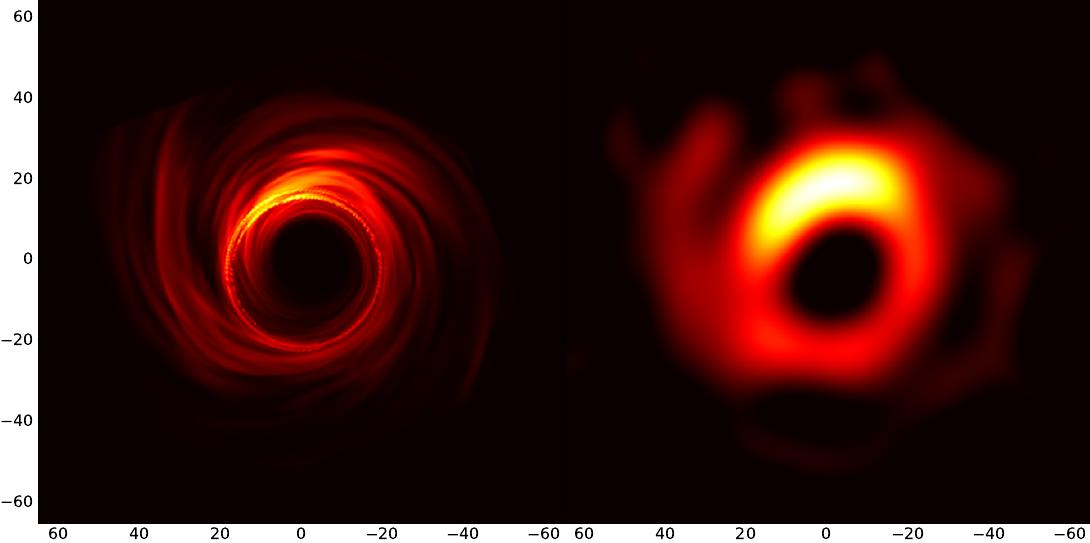
\includegraphics[scale=0.4]{figures/chapter1/m87_bh.jpeg}
        \caption{Left: Multi-dimensional general relativistic magneto-hydrodynamic simulation of the supermassive black hole located in the center of the M87 galaxy. Right: VLBI image reconstruction of the same black hole. Credit: \href{https://blackholecam.org/research/bhshadow/vlbi/}{Moscibrodzka (BHCAM, Radboud University), Akiyama (MIT)}.}
        \label{fig:m87_bh}
    \end{figure}

    Within the framework of general relativity, gravity is portrayed not as a force but as the warping of spacetime caused by the localized distribution of mass, according to Einstein's field equations:
    \begin{equation}\label{eq:gr_field_equation}
        R_{\mu \nu} - \frac{1}{2}g_{\mu \nu}R + \Lambda g_{\mu \nu} = \frac{8\pi G}{c^4} T_{\mu \nu}, 
    \end{equation}
    where $R_{\mu \nu}$ is the Ricci tensor, $g_{\mu \nu}$ is the metric tensor describing the geometry of the spacetime manifold, $R$ is the scalar curvature, $\Lambda$ is the cosmological constant\footnote{The cosmological constant was introduced by Einstein to allow for a static universe (though he later considered it his ``biggest blunder'' after the expansion of the universe was discovered). It is now understood to be related to dark energy.}, $T_{\mu \nu}$ is the stress-energy tensor, $G$ is the gravitational constant, and $c$ is the speed of light in a vacuum. Applying some tensor calculus, we can derive the Schwarzschild solution that describes the spacetime geometry surrounding a spherically symmetric (where $T_{\mu \nu} = 0$), non-rotating, and uncharged mass\footnote{The study of more complex systems that consider rotation and/or electric charge lead to other solutions, such as the Kerr and Reissner-Nordstr\"om solutions.}. The spacetime interval\footnote{A scalar quantity that generalizes the notion of distance from Euclidean space to curved spacetime. Also often called ``metric interval'' or simply ``metric''.} of the Schwarzschild solution is given by:
    \begin{equation}\label{eq:schwarzschild_metric}
        ds^2 = -\left(1 - \frac{2GM}{c^2r}\right)c^2dt^2 + \left(1 - \frac{2GM}{c^2r}\right)^{-1}dr^2 + r^2(d\theta^2 + \sin^2\theta d\phi^2),
    \end{equation}
    where $M$ is the mass of the object, $r$ is the radial coordinate, $t$ is the time coordinate, and $\theta$ and $\phi$ are the angular coordinates. 

    Often it is more convenient to express the Schwarzschild metric using the metric tensor, $g_{\mu \nu}$, in spherical coordinates:
    \begin{equation}\label{eq:schwarzschild_metric_matrix}
        g_{\mu\nu} = 
        \begin{pmatrix}
        -\left(1 - \frac{2GM}{c^2r}\right) & 0 & 0 & 0 \\
        0 & \left(1 - \frac{2GM}{c^2r}\right)^{-1} & 0 & 0 \\
        0 & 0 & r^2 & 0 \\
        0 & 0 & 0 & r^2\sin^2\theta \\
        \end{pmatrix},
    \end{equation}
    so that Eq.~\eqref{eq:schwarzschild_metric} can be written as:
    \begin{equation}\label{eq:schwarzschild_metric2}
        ds^2 = g_{\mu \nu}dx^\mu dx^\nu.
    \end{equation}
    The components of the metric tensor for the Schwarzschild solution illustrate in a concise manner how distances and times are altered due to the presence of a massive object: The time component, $g_{tt} = -\left(1 - \frac{2GM}{c^2r}\right)$, indicates the time dilation due to gravity; the radial component, $g_{rr} = \left(1 - \frac{2GM}{c^2r}\right)^{-1}$, shows the spatial distortion near the massive object; the angle components, $g_{\theta\theta} = r^2$ and $g_{\phi\phi} = r^2\sin^2\theta$, reflect the spherical symmetry of the spacetime around the massive object. 

    So far, in our discussion on the Schwarzschild solution, we have never mentioned black holes explicitly. In fact, all solutions stemming from Eq.~\eqref{eq:gr_field_equation} are not limited to describing black holes but are relevant to \textit{any} mass distribution. They are being used in a wide variety of applications, from calculating the precession of planetary orbits to improving the accuracy of the Global Positioning System (GPS). However, one may notice that the coefficient of the radial component of the metric tensor becomes infinite when:
    \begin{equation}\label{eq:schwarzschild_radius}
        r \equiv r_s = \frac{2GM}{c^2},
    \end{equation}
    which indicates a point of no return. This radius is called the ``\textit{Schwarzschild radius}'' and defines the boundary of a black hole, known as the `\textit{`event horizon}''. Inside this radius, the spacetime curvature is so extreme that all paths, space-like and time-like, lead inevitably towards the singularity at the center. In other words, any matter or radiation falling past the event horizon is irrevocably drawn into the central singularity, effectively making them invisible and detectable only by their gravitational effects on surrounding matter and radiation.

    Until very recently, the only observational confirmation of the existence of black holes were based on indirect evidence such as accretion disks and the associated X-ray emissions, gravitational lensing, and the orbital motion of stars near the center of galaxies. However, the detection of gravitational waves by the Laser Interferometer Gravitational-Wave Observatory (LIGO) and the Virgo observatory has provided direct evidence of black holes and, notably, black hole mergers. Moreover, in April 2019, the Event Horizon Telescope (EHT) released the first-ever ``image'' of a black hole's event horizon, or more accurately, the shadow of the supermassive black hole in the center of the galaxy M87 (see Fig.~\ref{fig:m87_bh})\footnote{The EHT uses very long baseline interferometry (VLBI) techniques to achieve the necessary resolution to observe the event horizon's "shadow" against the backdrop of the glowing gas in the accretion disk.}. This image provided direct visual evidence of a black hole's existence, showcasing a central dark region (the shadow) surrounded by a ring-like structure of light emitted by particles accelerated in the intense gravity near the event horizon. Both LIGO/Virgo and EHT observations were monumental confirmations of the predictions made by general relativity regarding the nature of black holes and their impact on surrounding spacetime and matter.

    \subsection{Binary Evolution}\label{sec:ch1:binaries}
    The evolution of stars in binary systems represents a complex process that differs significantly from the evolution of single stars. When two stars are gravitationally bound in a binary system, they orbit around a common center of mass. This close relationship leads to interactions that can significantly change their evolutionary paths. These interactions may include the transfer of mass from one star to the other, phases where both stars share a common outer layer, and even situations where the two stars merge. Such processes can change the way stars evolve, leading to outcomes that are not seen in the evolution of solitary stars. For instance, binary systems can give rise to phenomena like X-ray binaries, blue stragglers, and type Ia supernovae. These phenomena are important for our understanding of how galaxies evolve and how we measure distances in the universe. In this section, we will explore how the presence of a companion star influences the evolution of stars, highlighting the key differences from the evolution of single stars.

    \subsection{Supernovae: Origins and Classification}\label{sec:ch1:transients}
    \subsubsection{Core-Collapse Supernovae}
    \subsubsection{Electron-Capture Supernovae}
    \subsubsection{Supernovae Type-I}
    \subsubsection{Supernovae Type-II}


    \section{The Structure of Neutron Stars}\label{sec:ch1:ns_struct}

    \subsection{Formation and Hydrostatic Equilibrium}

    \subsection{Structure and Equation of State}
    \subsection{Exotic Phases and a Third Family of Compact Stars}
    \subsubsection{Construction of the Phase Transition}

    \section{Pulsar Astronomy}\label{sec:ch1:pulsar_astro}
    The discovery of pulsars in 1967 provided the first observational evidence for the existence of neutron stars. The precise timing of pulsars allows us to study the properties of neutron stars, including their rotation rates, magnetic fields, and mass. We will explore...

    \subsection{Pulsar Emission}
    \subsection{Spin-Down of Pulsars}
    \subsection{Pulsar Timing}
    \subsubsection{Phase Transition Signal in Pulsar Timing}

    \section{Thesis Outline}
    



\end{document}